\documentclass{article}
\usepackage{graphicx}
\graphicspath{ {./img/} }
\usepackage{amsmath}
\usepackage{amsfonts}
\usepackage{amssymb}
\usepackage{mathtools}
\usepackage[dvipsnames]{xcolor}
\usepackage{tkz-euclide}
\usepackage{subfiles}
\usepackage[left=1.5cm, right=1.5cm, top=1.5cm, bottom=1.5cm]{geometry}

\graphicspath{ {./img/} }

\usepackage{hyperref}
\hypersetup{
    colorlinks,
    citecolor=black,
    filecolor=black,
    linkcolor=black,
    urlcolor=black
}

\renewcommand\fbox{\fcolorbox{red}{white}}

\newcommand{\R}{\mathbb{R}}
\newcommand{\serie}{\sum_{n=1}^{+\infty}}

\title{Analisi Teoremi e Dimostrazioni Esame}
\author{Andrea Bellu}
\date{2023/2024}

\begin{document}

\maketitle

\tableofcontents

\section{Assiomi dei numeri reali}\
\begin{itemize}
    \item Assiomi relativi alle operazioni
    \item Assiomi relativi all'ordinamento
    \item Assioma di completezza
\end{itemize}

\subsection{Assiomi relativi alle operazioni}
Sono definite le operazioni di addizione e moltiplicazione tra coppie di numeri
reali e valgono le proprietà:
\begin{itemize}
    \item \textbf{Proprietà associativa}
    \item \textbf{Proprietà commutativa}
    \item \textbf{Proprietà distributiva}
    \item \textbf{Esistenza degli elementi neutri}
    \item \textbf{Esisstenza degli opposti}
    \item \textbf{Esistenza degli inversi}
\end{itemize}

\subsection{Assiomi relativi all'ordinamento}
E' definita la relazione di Minore o Uguale $\leq$.
\begin{itemize}
    \item \textbf{Dicotomia}
    \item \textbf{Proprietà Assimetrica}
    \item \textbf{Assioma di completezza}
\end{itemize}

\subsubsection{Assioma di completezza}
\[
    \forall a \in A, \forall b \in A, a \leq b  \implies \exists c \in A : a \leq c \leq b
\]
\newpage
\textbf{Esempi:}\\
\begin{figure}[h]
    \centering
    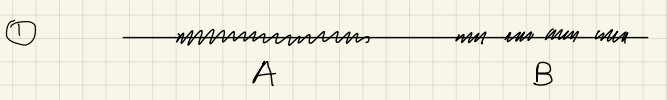
\includegraphics[width=0.3\textwidth]{1.png}
    \caption{Esempio 1}
    \label{fig:1}
\end{figure}

Esistono infiniti c.

\begin{figure}[!ht]
    \centering
    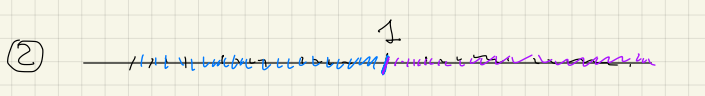
\includegraphics[width=0.3\textwidth]{2.png}
    \caption{Esempio 2}
    \label{fig:2}
\end{figure}
\[
    A = \{x \in \R : x \geq 1\} \ \ \ B = \{x \in \R : x \geq 1\} \implies c = 1
\]
\textbf{Osservazione:} Non tutti gli insiemi hanno il più grande o il più piccolo elemento. Ad esempio:
\[
    A = \{1, \frac{1}{2}, \frac{1}{3}, \frac{1}{4}, \cdots, \frac{1}{n}, \cdots\} = \{\frac{1}{n} : n\in \mathbb{N}\}
\]
\begin{figure}[h]
    \centering
    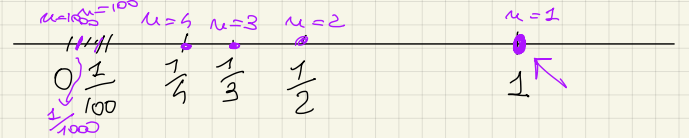
\includegraphics[width=0.3\textwidth]{3.png}
    \caption{Esempio 3}
    \label{fig:3}
\end{figure}

Non ha un elemento più piccolo. (Invece c'è il più grande che è $1$).

\subsection{Denso}
Si dimostra che $\mathbb{Q}$ è denso sulla retta reale (nel senso che fra due
numeri razionali è sempre possibile trovare un terzo, anzi infiniti).

\[
    a = \frac{m_1}{n_1} \ \ \ b = \frac{m_2}{n_2}
\]
faccio la media $\frac{a+b}{2} =\frac{\frac{m_1}{n_1} + \frac{m_2}{n_2}}{2} =
    \frac{m_1n_2 + m_2n_1}{2n_1n_2} \implies \in \mathbb{Q}$

\subsubsection{$\sqrt{2}$}
$\sqrt{2}$ non si può rappresentare come numero razionale.\\
\textbf{Dimostrazione:} Ragioniamo per assurdo, supponiamo che $\sqrt{2}$ sia un numero razionale, cioè $\sqrt{2} = \frac{m}{n}$ con $m,n \in \mathbb{Z}$ posso supporre che $m. n$ siano primi tra loro e che al più uno tra loro sia pari.
Allora $2 = \frac{m^2}{n^2} \implies  2n^2 = m^2 (\star)$\\
$\implies m^2$ deve essere pari e quindi $m$ è pari.\\
Posso esprimere $m$ nella forma: $m = 2k$ con $k$ intero.\\
Ricavo che $\implies 2n^2 = m^2 = 4k^2$ semplifico per $2$ e ottengo $n^2 = 2k^2$\\
Ripeto il ragionamento precedente $\implies n^2$ pari e quindi anche $n$ pari. Ma allora sia $m$ che $n$ risultano pari, ASSURDO!\\
Avevo supposto che fossero primi ed (al più) uno dei due pari. $\clubsuit$

Per capire meglio guarda esempi della Francy nella prima lezione.

\section{Complementi ai numeri reali}
\subsection{Massimo, Minimo, Estremo Superiore, Estremo Inferiore}
\[
    \text{Def: M è il massimo di A} \begin{cases}
        M \in A  \ \ (1) \\
        M \geq a \ \ \forall a \in A \ \ (2)
    \end{cases}
\]
Il massimo di un insieme di numeri reali $A$ quindi, se esiste, è un numero $M$
dell'insieme $A$, che è maggiore o uguale ad ogni altro elemento dell'insieme
$A$.
\[
    \text{Def: m è il minimo di A} \begin{cases}
        m \in A  \ \ (1) \\
        m \leq a \ \ \forall a \in A \ \ (2)
    \end{cases}
\]
Il minimo di $A$ analogamente, se esiste, è un numero $m$ di $A$, che è minore
o uguale ad ogni altro elemento di $A$.

\subsubsection{Il massimo e il minimo sono unici}
Il massimo e il minimo, se esistono, sono unici.\\ \textbf{Dimostrazione:}
Siano $M_1$ e $M_2$ due massimi di $A$.\\ Ma allora per definizione di massimo,
\[
    (1) \ M_1 \geq a \ \ \ \ (2) \ M_2 \geq a \ \ \ \ \forall a \in A
\]
Sempre per definizione, $M_1, M_2$ sono elementi di $A$.\\ Quindi da $(1)$ se
$a = M_2$, ottengo $M_1 \geq M_2$\\ Da $(2)$ se $a = M_1$, ottengo $M_2 \geq
    M_1$\\ Segue che $M_1 = M_2$ $\clubsuit$.

\subsubsection{Osservazione}
Un insieme finito ammette sempre massimo e minimo, ma consideriamo i seguenti
insiemi:
\begin{itemize}
    \item $A = \{\frac{1}{n} : n\in \mathbb{N}\}$, il più grande elemento di $A$ è $1$, che è il massimo, il più piccolo non c'è.
    \item $B = \{1-\frac{1}{n} : n\in\mathbb{N}\} = \{\frac{n-1}{n} : n\in\mathbb{N}\}$, il più piccolo elemento di $B$ è $0$, che è il minimo, il più grande non c'è.
\end{itemize}

\subsection{Maggiorante e Minorante}
$L$ si dice \textbf{maggiorante} per un insieme $A$ se
\[
    L \geq a \ \ \ \ \forall a \in A
\]
$l$ si dice \textbf{minorante} per un insieme $A$ se
\[
    l \leq a \ \ \ \ \forall a \in A
\]
\textbf{Non} sempre un insieme $A$ ammette maggioranti e minoranti.\\
L'insieme $A$ si dice \textbf{limitato superiormente} se ammette un maggiorante.\\
L'insieme $A$ si dice \textbf{limitato inferiormente} se ammette un minorante.\\
L'insieme $A$ si dice \textbf{limitato} se è limitato superiormente ed inferiormente, in simboli:
\[
    l\leq a \leq L \ \ \ \ \forall a \in A \implies \exists M : |a| \leq M \ \ \ \ \forall a \in A
\]

\subsection{Teorema dell'esistenza dell'estremo superiore}
Sia $A$ un insieme non vuoto di numeri reali e limitato superiormente. Allora
esiste il minimo dell'insieme dei maggioranti di $A$.
\[
    A = \{a\in A\} \ \ \ \ B = \{b \text{ maggiorante di } A\}
\]
Applichiamo l'assioma di completezza di due insiemi $A$ e $B$, quindi esiste
$c$ numero reale tale che:
\[
    a \leq c \leq b \ \ \ \ \forall a \in A \ \ \ \ \forall b \in B
\]
Dato che $c \geq a \ \ \ \ \forall a \in A$, $c$ è un maggiorante di $A$, cioè
$c \in B$.\\ Ma $c$ è anche tale che $c\leq b$ (minore o uguale a tutti gli
elementi di $B$). $\implies c$ è un minimo. $\clubsuit$\\ Allora possiamo dare
la seguente definizione:\\
\subsubsection{Estremo superiore}
\textbf{Def:} Sia $A$ un insieme non vuoto di numeri
reali e limitato superiormente. Diremo che $M\in \R$ è l\textbf{'estremo
    superiore} di $A$ se $M$ è il minimo dei maggioranti di $A$. In simboli:
\[
    M \text{ estremo superiore di } A \iff \begin{cases}
        M \geq a  \ \ \ \ \forall a \in A \ \ (\textbf{1}) \text{ (M è maggiorante)} \\
        \forall \varepsilon > 0 \ \ \ \ \exists a \in A : M - \varepsilon < a \ \ (\textbf{2}) \text{ (M è il minimo dei maggioranti)}
    \end{cases}
\]
Analogamente:
\subsubsection{Estremo inferiore}
\textbf{Def:} Sia $A$ un insieme non vuoto di numeri reali e limitato inferiormente. Diremo che $m$ è l'\textbf{estremo inferiore} di $A$ se $m$ è il massimo dei minoranti di $A$. In simboli:
\[
    m \text{ estremo inferiore di } A \iff \begin{cases}
        m \leq a  \ \ \ \ \forall a \in A \ \ (\textbf{1}) \text{ (m è minorante)} \\
        \forall \varepsilon > 0 \ \ \ \ \exists a \in A : m + \varepsilon > a \ \ (\textbf{2}) \text{ (m è il massimo dei minoranti)}
    \end{cases}
\]
$\implies$ Quindi se un insieme è limitato superiormente allora esiste l'estremo superiore ed è un numero reale. Se un insieme è limitato inferiormente, allora esiste l'estremo inferiore ed è un numero reale.
Altrimenti:
\begin{itemize}
    \item L'estremo superiore è $+\infty$ se $A$ non è limitato superiormente
    \item L'estremo inferiore è $-\infty$ se $A$ non è limitato inferiormente
\end{itemize}
\[
    \begin{cases}
        \sup A = +\infty \iff \forall M \in \R \ \ \ \ \exists a \in A : M < a \\
        \inf A = -\infty \iff \forall m \in \R \ \ \ \ \exists a \in A : m > a
    \end{cases}
\]

\end{document}